
\begin{figure}[ht]
\footnotesize
\begin{tabular} {|p{0.7\linewidth}|c|} 
    \hline
    $\finchlookup(seek, body)$: The Lookup looplet represents a randomly accessible region of an iterator. The body of the lookup is understood to have one less dimension than the lookup itself, as we have already ``looked up'' that index in the tensor by the time we reach the body. \texttt{seek(i)} is a function that updates state to the given index.
    &
    \raisebox{-0.85\totalheight}{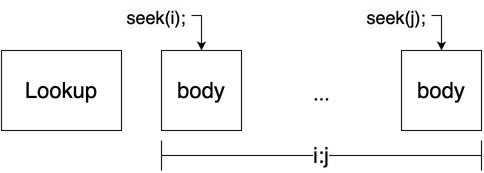
\includegraphics[scale=0.20]{Looplets-lookup.png}}
    \\
    \hline
    $\finchrun(body)$: The Run looplet represents a constant region of an iterator. The body of the run is understood to have one less dimension than the lookup itself, as all of the bodies are identical.
        &
    \raisebox{-0.85\totalheight}{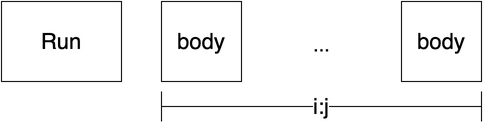
\includegraphics[scale=0.20]{Looplets-run.png}}
    \\ 
    \hline
    $\finchphase(c:d, body)$: The Phase looplet represents a restriction of the range on which a loop should execute, and allows us to succinctly express the ranges on which children of compound looplets are defined.
    &
    \raisebox{-0.85\totalheight}{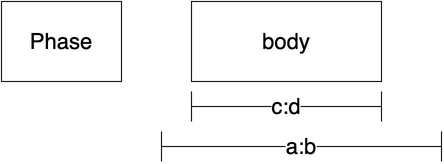
\includegraphics[scale=0.20]{Looplets-phase.png}}
    \\ 
    \hline
    $\finchswitch(cond, head, tail)$: The Switch looplet allows us to specialize the body of a looplet based on a condition, evaluated in the embedding context. If the condition is true, we use `head`, otherwise we use `tail`. Switch has a high lowering priority so we can see what's inside of it and lower that appropriately. This also lifts the condition as high as possible into the loop nest. The condition is assumed to evaluate to a Boolean.
    &
    \raisebox{-1\totalheight}{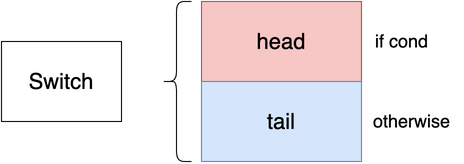
\includegraphics[scale=0.20]{Looplets-switch.png}}
    \\ 
    \hline
    $\finchthunk(preamble, body, epilogue)$: The Thunk looplet allows us to cache certain computations in the state under which the body will execute. This is useful for computing and caching the results of expensive computations.
    &
    \raisebox{-0.8\totalheight}{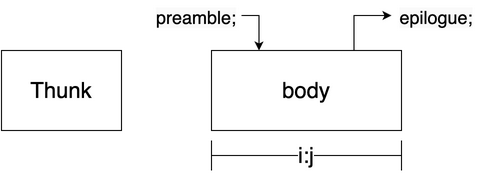
\includegraphics[scale=0.20]{Looplets-thunk.png}}
    \\ 
    \hline
    $\finchsequence(head, tail)$: The Sequence looplet represents the concatenation of two looplets. Both arguments must be phase looplets, and are assumed to be non-overlapping, covering, and in order.
    &
    \raisebox{-0.85\totalheight}{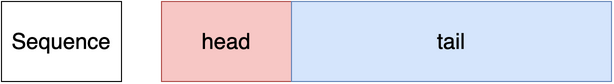
\includegraphics[scale=0.20]{Looplets-sequence.png}}
    \\ 
    \hline
    $\finchspike(body, tail)$: The Spike looplet represents a run followed by a single value. In this paper, Spike will be considered a shorthand for $\finchsequence(\finchphase(i:j-1, \finchrun(body)), \finchphase(j:j, \finchrun(tail)))$.  In the Finch compiler, spikes are handled with special care, since they are an opportunity to align the final run to the end of the root loop extent, without using any special bounds inference.
    &
    \raisebox{-1.15\totalheight}{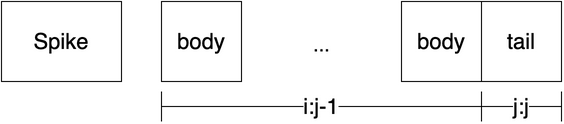
\includegraphics[scale=0.20]{Looplets-spike.png}}
    \\ 
    \hline
    $\finchstepper([seek], next, body)$: The stepper looplet represents a variable number of looplets, concatenated. Since our looplets may be skipped over due to conditions or various rewrites, the $seek$ function allows us to fast-forward the state to the start of the root loop extent when it comes time to lower the stepper. The $next$ function advances the state to the next iteration of the stepper. 
    &
    \raisebox{-1\totalheight}{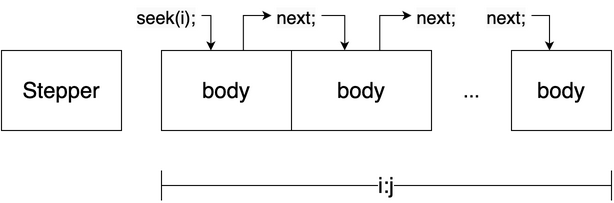
\includegraphics[scale=0.20]{Looplets-stepper.png}}
    \\
    \hline
    \end{tabular}
\vspace{-8pt}
\caption{The Looplet language, as understood in a correct execution of a Finch program.}\label{fig:looplets}
\end{figure}

\section{Background}

\subsection{Looplets}
Finch represents iteration patterns using Looplets, a language that decomposes datastructure iterators hierarchically. 
%
Looplets represent the control-flow structures needed to iterate over any given datastructure, or multiple datastructures simultaneously. 
%
In particular, Looplets are good at lifting code to the highest possible loop level and subdividing iteration hierarchically in coordinate space.
%
Because Looplets are compiled with progressive lowering, structure-specific mathematical optimizations such as integrals, multiply by zero, etc. can be implemented using simple compiler passes like term rewriting and constant propagation during the intermediate lowering stages.

The Looplets are described in Figure~\ref{fig:looplets}. We simplify the presentation to focus on the semantics, rather than precise implementation. Several looplets introduce or modify variables in the scope of the target language. It is assumed that if a looplet introduces a variable, the child looplet will not modify that variable. For more background on Looplets, we recommend the original work \cite{ahrens_looplets_2023}. 

\begin{wrapfigure}{r}{0.45\linewidth}
    \centering
    \vspace{-28pt}
    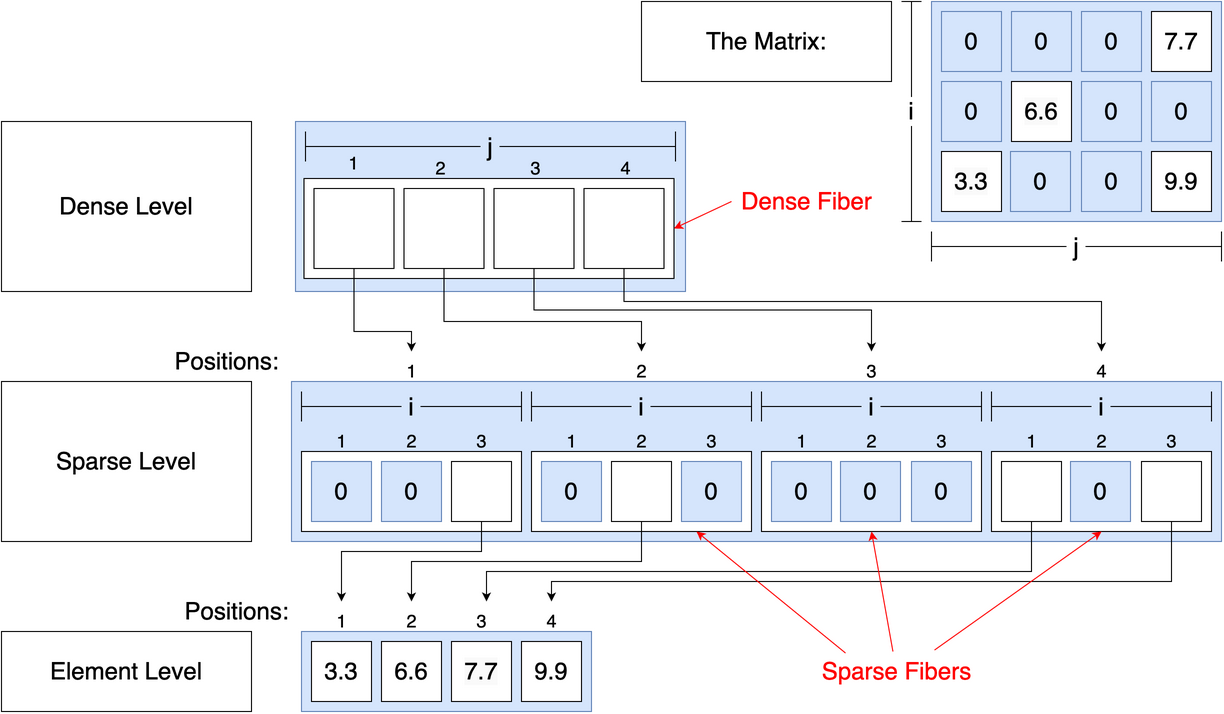
\includegraphics[width=\linewidth]{LevelsVsFibers-matrix.png}
    %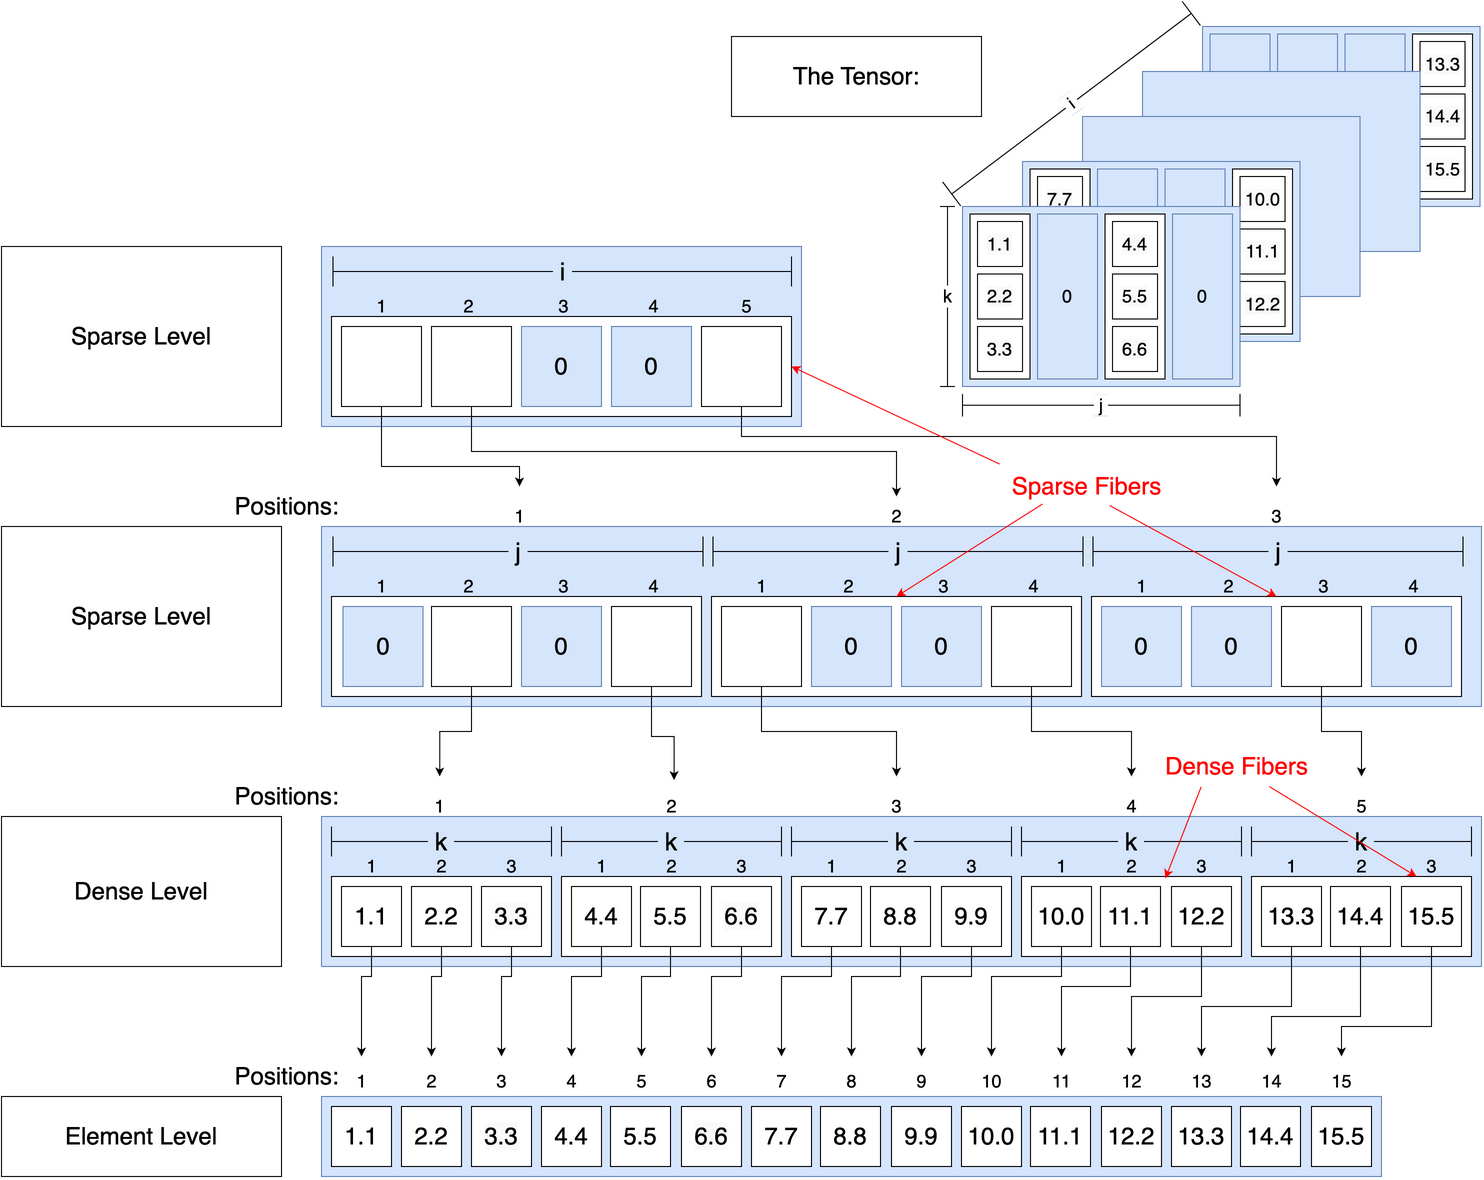
\includegraphics[width=0.5\linewidth]{LevelsVsFibers-tensor.png}
    \vspace{-16pt}
    \caption{Levels in the fiber tree representation of a sparse matrix in CSC format, with a dense outer level and a sparse inner level. The element level holds the leaves of the tree.}
    \label{fig:levelsvsfibers}
    \vspace{-24pt}
\end{wrapfigure}
\subsection{Fiber Trees}

Fiber-tree style tensor abstractions have been the subject of extensive study
\cite{sze2017efficient, chou2022compilation, chou2018format}.  The underlying
idea is to represent a multi-dimensional tensor as a nested vector
datastructure, where each level of the nesting corresponds to a dimension of the
tensor. Thus, a matrix would be represented as a vector of vectors. This kind of
abstraction lends itself to representing sparse tensors if we vary the type of
vector used at each level in a tree. Thus, a sparse matrix might be represented
as a dense vector of sparse vectors. The vector of subtensors in this
abstraction is referred to as a \textbf{fiber}.

Instead of storing the data for each subfiber separately, most sparse tensor
formats such as CSR, DCSR, and COO usually store the data for all fibers in a
level contiguously. In this way, we can think of a level as a bulk allocator for
fibers. Continuing the analogy, we can think of each fiber as being
disambiguated by a \textbf{position}, or an index into the bulk pool of
subfibers. The mapping $f$ from indices to subfibers is thus a mapping from an
index and a position in a level to a subposition in a sublevel.
Figure~\ref{fig:levelsvsfibers} shows a simple example of a level as a pool of fibers.

When we need to refer to a particular fiber at position $p$ in the level $l$, we
may write $fiber(l, p)$. Note that the formation of fibers from levels is lazy,
and the data underlying each fiber is managed entirely by the level, so the
level may choose to overlap the storage between different fibers. Thus, the only
unique data associated with $fiber(l, p)$ is the position $p$.